
\documentclass{AbstractTemplate}

\usepackage{graphicx}
\usepackage{epstopdf}

\title{Detecting the Chromatin Grammar of Active Transcription Factor Binding Sites}

\author{Eduardo G. Gusm\~{a}o\,\affref{ref1}$^{,}$\affref{ref3}, Christoph Dieterich\,\affref{ref2}, Martin Zenke\,\affref{ref3} and Ivan G. Costa\,\affref{ref1}$^{,}$\affref{ref3}$^{,*}$}

\affiliation{
  \aff{ref1}
  	{IZKF Aachen Computational Biology Research Group, Institute for Biomedical Engineering, RWTH Aachen University Medical School, Germany.}
  \aff{ref2}
  	{Computational RNA Biology and Ageing, Max Planck Institute for Biology of Ageing, Germany.}
  \aff{ref3}
  	{Department of Cell Biology, Institute for Biomedical Engineering, RWTH
Aachen University Medical School, Germany.}
  $^{*}$ ivan.costa@rwth-aachen.de
}

\begin{document}

\maketitle

\section{Introduction}
\label{sec:introduction}

Standard sequence-based approaches to find binding sites suffer from a high number of false positive hits. Among others, these methods are unable to identify sites which are active in a particular cellular context~\cite{boyle2011}. Current research has proven that novel genome-wide assays reflecting chromatin structure, such as DNase I Hypersensitivity (DHS -- obtained with DNase-seq) or particular histone modifications (obtained with ChIP-seq) can be combined with sequence-based methods to improve the detection of cell-specific transcription factor binding sites~\cite{boyle2011,neph2012a, pique2011,won2010}. For example, signal segmentation methods were applied to DNase-seq~\cite{boyle2011,neph2012a} to detect footprints, which indicate the location of active binding sites on a base pair resolution. Previously, ~\cite{won2010} proposed a similar approach to detected ``footprints'' with histones marks H3K4me1 and H3K4me3. These segmentation methods provide active regions, which can then be further analyzed with sequence-based approaches for detecting binding sites with known or novel motifs. A distinct strategy is performed by site-centric approaches~\cite{cuellar2012,pique2011}. These methods start with sequence-based predicted binding sites and classify them as active/inactive given their surrounding DHS and histone modification signals. So far, only~\cite{cuellar2012,pique2011} attempted to combine both DHS and histones to predict active binding sites. Interestingly, both studies found that DHS alone provides very good accuracy; while the addition of histone modifications did not provide substantial improvement.

\section{Method}
\label{sec:method}

We propose an HMM-based approach to integrate both DHS and histone modifications for the detection of open chromatin regions and active TFBSs. We and others have previously observed that the peak-dip-peak patterns of the DHS profile happen inside the dip of the histone modification profiles~\cite{gusmao2012,neph2012a,kundaje2012}. This indicates an underlying chromatin grammar behind active TFBSs: open chromatin regions (high DHS) are flanked by high or moderate signals of active histone marks. These open chromatin regions consist of a sequence of one or more footprints indicative of active TFBSs (low histone modification and DHS signals). We have therefore devised an HMM to model this epigenetic grammar by simultaneous analysis of DNase-seq and the ChIP-seq profiles of histone marks. Here, we use histone modifications/variants H3K4me1, H3K4me3, H3K9ac, H3K27ac and H2A.Z as they are indicative of active regulatory regions. This is the first approach combining local genomic profiles of histone modification and DHS for the detection of open chromatin and active TFBSs.

The method can be summarized as follows. First, we pre-process the signals from the DNase-seq and ChIP-seq experiments obtained from the ENCODE repository~\cite{encode2012}. We apply a two-step normalization process that addresses both within- and between-dataset variability. We also estimated the slope of the genomic signals to be able to detect increase and decrease on the signals. Both normalized and slope signals for DHS and histone modifications are used as input for our multivariate HMM, which was designed to detect the underlying epigenetic grammar of active TFBSs. The HMM is trained with signal from a manually annotated genomic region. Then, the HMMs are applied to genome-wide DHS and histone modification signals. The output, i.e. footprints, represents regions likely to be active binding sites for TFs.

\section{Results}
\label{sec:results}

In order to validate our and competing methods we created a site-centric validation set as~\cite{cuellar2012}. We obtained ChIP-seq experiments from 83 TFs for cell types H1-hESC and K562 from ENCODE. Then, we find all motif-predicted binding sites (MPBSs) for all TFs in the genome using Position Weight Matrices (PWMs) obtained in Jaspar~\cite{mathelier2014}, Transfac~\cite{matys2006} and Uniproble~\cite{robasky2011} repositories. All MPBSs that overlapped ChIP-seq enriched regions are considered `true' TFBSs; otherwise it is a `false' TFBS. By overlapping such validation set with the predictions made by all methods, we are able to create a Receiver Operating Characteristic (ROC) curves and calculate their respective Area Under the ROC Curves (AUC) for each TF.

The Fig.~\ref{fig:boxplot} show the AUC distribution over all 83 TFs tested for the following methods: our DHS+histone HMMs with either 2 (`DH-HMM (2)`) or 3 (`DH-HMM (3)`) histone modifications, `Centipede'~\cite{pique2011}, `Neph'~\cite{neph2012a}, `Cuellar'~\cite{cuellar2012}, `Boyle'~\cite{boyle2011}, a histone-only version of our method (`H-HMM') and a purely sequence-based method (`PWM'). The numbers indicated in some method's labels represent the number of histones used to create the predictions. At first glance we are able to observe that all methods outperform the sequence-based TFBS detection (`PWM'). In order to test all methods with regard to their AUC distribution, we performed a Friedman-Nemenyi test. We observed that our method significantly outperformed all other methods ($p$-value $< 0.05$). 
\begin{figure*}[h!]
\centering
     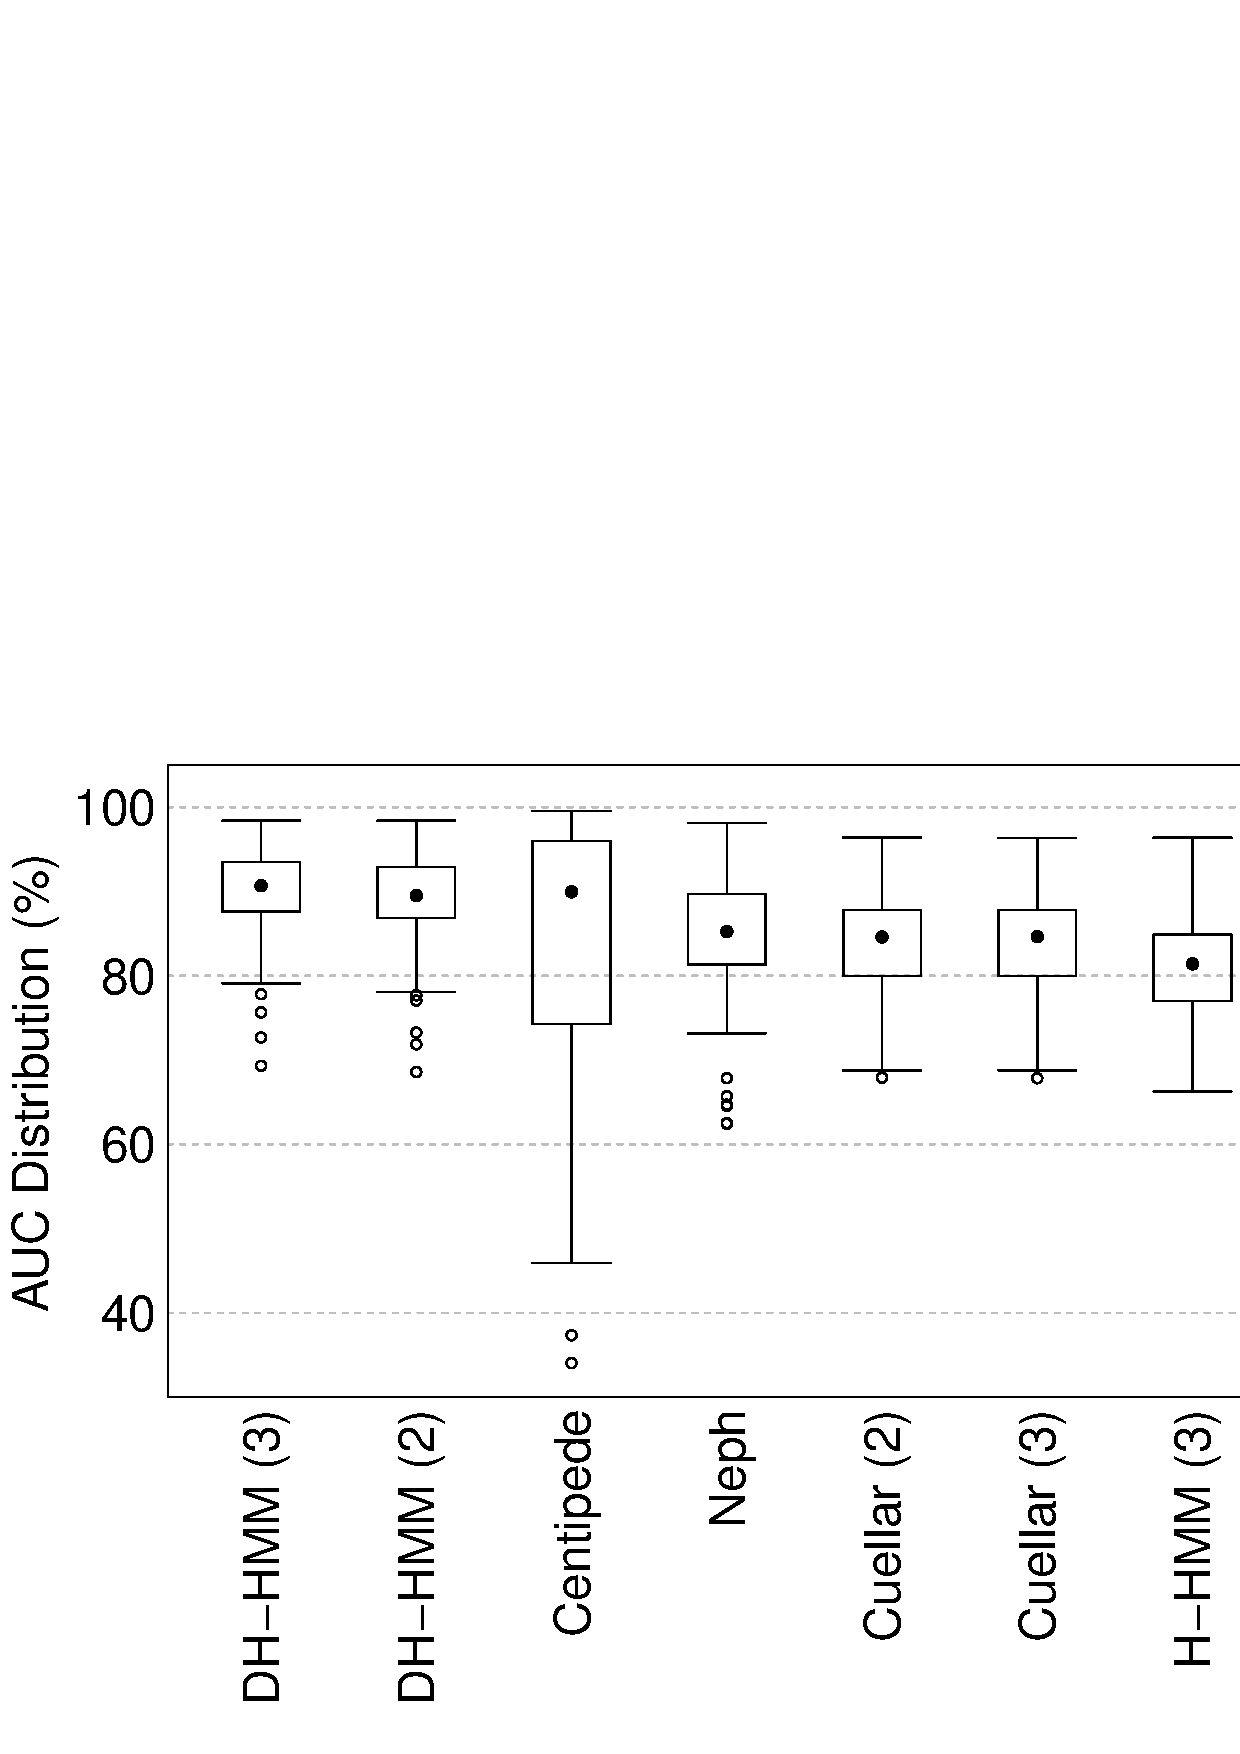
\includegraphics[width=0.95\textwidth]{Figure/boxplot}
\caption{AUC distribution for our (DH-HMM) and competing methods over a validation set of 83 TFs. The methods are sorted in an increasing manner, from left to right, according to their Friedman ranking.}
\label{fig:boxplot}
\end{figure*}

Moreover, we also performed further experiments to assess our model. First, we evaluated all combinations (up to three) of the 5 histone marks previously mentioned. Results show that using more marks improves AUC and that several combination of marks are equally good. Also, we evaluated the performance of the HMM after training and applying it in data from four distinct cell types. Results show that there is insignificant difference in the AUC values. This indicates that	 the chromatin grammar is common to all cells analyzed. Finally, among all segmentation-based methodologies, our technique has provided the best spatial specificity, i.e. the predictions are closer to active TFBSs.

\paragraph{Funding:}
This work was supported by the Interdisciplinary Center for Clinical Research
(IZKF Aachen), RWTH Aachen University Medical School, Aachen, Germany; and Brazilian research
agencies: FACEPE and CNPq.

\bibliographystyle{AbstractTemplate}
{\footnotesize
\bibliography{document}}

\end{document}
